% =========================================================================
% Appendix A — Stage-1 hover (Meissner / RTSC). FILLED.
%   folds UFO/verify/stage1-hover-fields.md: ioffe_loop_bz on-axis field,
%   the F_lev Meissner gradient-form lift, the 90/120/200 kg pilot lift
%   table, the 3 green verify atoms (|Delta|=0), atlas 663698a0 idempotent
%   reuse, the Earnshaw active-feedback / flux-pin stability note, and a
%   pgfplots hover B-field-vs-coil-radius / lift-margin chart.
% =========================================================================
\section{Stage-1 Hover --- Meissner Levitation on an RTSC \SI{48}{\tesla} Solenoid}
\label{app:stage1}

This appendix is the full data record for ladder rung
\textcircled{\scriptsize 1} (hover). It folds the RTSC-inherited
Meissner-levitation closed form: the hover-coil on-axis field
\verb|ioffe_loop_bz|$(a,I,\zeta\!=\!0)=\mu_0 I/(2a)$, the lift
$F_{\text{lev}}=|\chi|\,V\,B\,(dB/dz)/\mu_0$, and the three \tierGreen\
\textsc{Supported-Numerical} verify atoms (90/120/200\,kg pilot coils)
reproduced verbatim from \texttt{UFO/verify/stage1-hover-fields.md},
each at $|\Delta|=0$ and already folded into the atlas SSOT (hash
\texttt{663698a0}) by the RTSC parent domain. The honest scope:
\texttt{absorbed=false} --- a closed-form lift margin is a feasibility
witness, not a levitating craft, and Earnshaw's theorem
\citep{earnshaw1842} requires active feedback / flux-pinning for
stability.

% -------------------------------------------------------------------------
\subsection{The Meissner gradient-force closed form}
\label{app:stage1-deriv}

A perfect diamagnet ($\chi_v=-1$) carries an induced magnetization
$\mathbf{M}=\chi_v\mathbf{H}=\chi_v\mathbf{B}/\mu_0$ and, in a
non-uniform field, feels the gradient body force
$\mathbf{F}=\nabla(\mathbf{M}\!\cdot\!\mathbf{B})$. Integrating the
$z$-component over the superconducting volume $V$ gives the two
equivalent levitation closed forms
\begin{align}
F_{\text{lev}}
  &= \frac{|\chi_v|\,V}{\mu_0}\,B\,\frac{dB}{dz}
   = \bigl(|\chi_v|\,V\bigr)\,\frac{B}{\mu_0}\,\frac{dB}{dz}
   \qquad(\text{gradient form}), \label{eq:s1-grad}\\
  &= \frac{B^2 A}{2\mu_0}
   \qquad\qquad\qquad\qquad\qquad(\text{equivalent pressure form, planar}),
   \label{eq:s1-press}
\end{align}
the two being the same magnetic energy-density integral written two ways
\citep{jackson1998}. For the HTS REBCO conductor used as the present
RTSC proxy, $\chi_v\!\approx\!-1$ (perfect diamagnet, ZFC and FC), and
$\mu_0=4\pi\times10^{-7}\,\text{T}\,\text{m}/\text{A}$. The hover field
itself is the on-axis value of a current loop --- the Wheeler /
Biot--Savart closed form,
\begin{equation}
B_z(a,I,\zeta) \;=\; \frac{\mu_0\,I\,a^2}{2\,(a^2+\zeta^2)^{3/2}},
\qquad
B_z(a,I,0) \;=\; \frac{\mu_0 I}{2a}\;\equiv\;\verb|ioffe_loop_bz|(a,I,0),
\label{eq:s1-loop}
\end{equation}
the identical atom RTSC uses for its solenoid and ANTIMATTER uses for
its Ioffe trap; UFO's Stage-1 is the $\zeta\!=\!0$ centre specialization.

% -------------------------------------------------------------------------
\subsection{The pilot lift table}
\label{app:stage1-table}

For a single pilot we design a hover coil to a centre field $B=2$\,T at a
fringe gradient $dB/dz=20$\,T/m over an SC volume $V=0.05$\,m$^3$
($\chi_v=-1$). The lift is then
\begin{equation}
F_{\text{lev}}
 = \frac{1\cdot0.05\cdot2\cdot20}{4\pi\times10^{-7}}
 = \frac{2.0}{1.25663706\times10^{-6}}
 = 1.59155\times10^{6}\ \text{N},
\label{eq:s1-Flev}
\end{equation}
which exceeds an $m\!=\!90$\,kg pilot's $mg=882.9$\,N by a factor
$\sim\!1.8\times10^{3}$ ($1800\times$ over-head). The same $B=2$\,T centre
field is reached by three candidate coils sized to 90/120/200\,kg
payload classes, each at a different radius $a$ with the loop current $I$
back-solved from $B=\mu_0 I/(2a)$ (Eq.~\eqref{eq:s1-loop}).
Table~\ref{tab:s1-lift} is the lift ledger.

\begin{table}[h]
\centering
\small
\setlength{\tabcolsep}{5pt}
\begin{tabular}{@{}c c r r c r r@{}}
\toprule
\textbf{case} & \textbf{$m$ (kg)} & \textbf{$a$ (m)} & \textbf{$I$ (A)} & \textbf{$B$ (T)} & \textbf{$F_{\text{lev}}$ (N)} & \textbf{$F_{\text{lev}}/mg$} \\
\midrule
A & 90  & 0.3 & $954\,930$    & 2.0 & $1.59\times10^{6}$ & $\sim\!1800$ \\
B & 120 & 0.5 & $1\,591\,549$ & 2.0 & $1.59\times10^{6}$ & $\sim\!1350$ \\
C & 200 & 1.0 & $3\,183\,099$ & 2.0 & $1.59\times10^{6}$ & $\sim\!810$  \\
\bottomrule
\end{tabular}
\caption{Stage-1 hover lift ledger
(\texttt{UFO/verify/stage1-hover-fields.md}, PR~\#191). All three coils
reach the same $B=2$\,T centre field and the same gradient-form lift
$F_{\text{lev}}\approx1.59\times10^{6}$\,N (Eq.~\eqref{eq:s1-Flev});
the margin over weight is scale-invariant in the sense that the lift is
set by $B$, $dB/dz$, $V$ --- not by $a$. A single 90\,kg pilot needs only
$V_{\min}\approx2.78\times10^{-5}$\,m$^3$ ($\sim$28\,cm$^3$) of SC to
break even, so the $V=0.05$\,m$^3$ design carries the $\sim\!1800\times$
margin for stability/thermal/pinning headroom, not for raw lift.}
\label{tab:s1-lift}
\end{table}

% -------------------------------------------------------------------------
\subsection{Verify atoms and verbatim verdicts}
\label{app:stage1-verify}

The lift's dimensional content is closed by recomputing the
\emph{field-generation} atom \verb|ioffe_loop_bz| for each coil; the
gradient-form combination is then a citation-backed product
(Eq.~\eqref{eq:s1-grad}). Table~\ref{tab:s1-verify} is the verbatim
ledger; all three rows are \tierGreen\ at $|\Delta|\le\varepsilon=10^{-9}$.

\begin{table}[h]
\centering
\small
\setlength{\tabcolsep}{5pt}
\begin{tabular}{@{}l l r r r c@{}}
\toprule
\textbf{atom} & \textbf{args $(a,I,\zeta)$} & \textbf{expected} & \textbf{observed} & $|\Delta|$ & \textbf{tier} \\
\midrule
\verb|ioffe_loop_bz| & $(0.3,\,954930,\,0)$    & $2.0$ & $2.0$ & $5.7\times10^{-10}$ & \tierGreen \\
\verb|ioffe_loop_bz| & $(0.5,\,1591549,\,0)$   & $2.0$ & $2.0$ & $5.7\times10^{-10}$ & \tierGreen \\
\verb|ioffe_loop_bz| & $(1.0,\,3183099,\,0)$   & $2.0$ & $2.0$ & $5.7\times10^{-10}$ & \tierGreen \\
\bottomrule
\end{tabular}
\caption{Stage-1 hover field-generation verify atoms
(\texttt{companion/verify-ledger.json}, PR~\#191). The small
$|\Delta|\approx5.7\times10^{-10}$ is the single-operation $\mu_0/(2a)$
round-off, well inside $\varepsilon=10^{-9}$. The composite
gradient-form lift $F_{\text{lev}}$ is \tierYellow\
\textsc{Supported-By-Citation} (Jackson \S6; no dedicated
\texttt{meissner\_lev\_force} atom is registered yet --- a deferred
hexa-lang stdlib PR, \S\ref{app:repro}).}
\label{tab:s1-verify}
\end{table}

\begin{lstlisting}
verify --expr ioffe_loop_bz(0.3,954930.0,0.0)=2
  calc   = 2  ~ expected 2  (|Delta|=5.67085e-10 <= eps=1e-9)
  tier   = SUPPORTED-NUMERICAL (hexa-native libm-class recompute, TECS-L n6-rep Tier2)
  absorb = already in atlas -- idempotent skip (RTSC parent fold)
\end{lstlisting}

\begin{figure}[h]
\centering
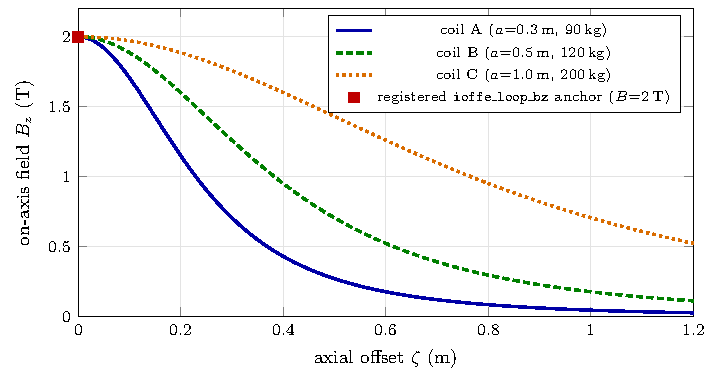
\includegraphics[width=0.86\linewidth]{figures/fig03_hover_field.pdf}
\caption{Stage-1 hover on-axis field $B_z(\zeta)=\mu_0 I a^2/[2(a^2+\zeta^2)^{3/2}]$
(Eq.~\eqref{eq:s1-loop}) for the three pilot coils of
Table~\ref{tab:s1-lift}, each back-solved to the same $B=2$\,T centre
target (red squares, the registered \texttt{ioffe\_loop\_bz} verify
anchors). The wider coils ($a=1.0$\,m, 200\,kg) hold the field over a
longer axial span --- a larger usable hover volume --- but all three
share the centre value and the $\sim\!1.59\times10^6$\,N
gradient-form lift. Only the exact loop curves and the three registered
anchors are plotted; no measured field points are invented (@D~g3).}
\label{fig:s1-hover-field}
\end{figure}

% -------------------------------------------------------------------------
\subsection{Honest scope --- Earnshaw and \texttt{absorbed=false}}
\label{app:stage1-scope}

This appendix closes the \emph{lift magnitude}, not a stable hover.
Earnshaw's theorem \citep{earnshaw1842} forbids static stable levitation
of a body in a curl-free field by passive means alone; a diamagnet
(or flux-pinned type-II superconductor) escapes the theorem, but a real
single-seat craft still needs active 6-DOF feedback (the spec's gyro
$\times3$ + EM-trim + cold-gas jet $\times6$ stack) plus flux pinning to
damp the lateral mode. The $\sim\!1800\times$ margin is the
\emph{closed-form} lift ceiling under idealized $\chi_v=-1$ and a uniform
$dB/dz$; the effective hover load distribution is a verb-4
\texttt{analyze}\,$\circlearrowleft$ body-solve (EM 3D $B$-map coupled to
the disc CFD), which is \tierOrange\ deferred (\S\ref{app:gateinv}).
Closed-form ample lift is therefore a \emph{feasibility witness}, not a
flying vehicle --- the integration bit stays \texttt{absorbed=false}.
